\documentclass[11pt,a4paper]{scrbook} 
\usepackage[utf8]{inputenc}
\usepackage{amsmath}
\usepackage{amsfonts}
\usepackage{amssymb}
\usepackage{graphicx}
\usepackage{longtable}
\usepackage{multirow}
\renewcommand{\familydefault}{\sfdefault}
\usepackage{droid}
\usepackage[left=2cm, right=2cm, top=1cm, bottom=2cm]{geometry}
\usepackage{ngerman}
\usepackage{tabularx}
\usepackage{graphicx}
\usepackage{enumitem}
\usepackage{scrpage2}	%Kopf- und Fußzeile
\usepackage{picinpar}	%Textumläufe von Grafiken
\usepackage{pdfpages}	%Implementierung von pdf als ganze Seite(Seiten sind nicht editierbar)
\usepackage{lastpage}	%Implmentiert 'letzte Seite', wird für Kopfzeile benötigt
\usepackage{listings}


\usepackage{lastpage}




\pagestyle{scrheadings}


\ifoot{\ \copyright Noah Kofort, Klaus Suthe - v0.2} \setfootsepline{1pt}\ofoot{ \thepage \  von \pageref{LastPage}\ }

\begin{document}

\raggedleft
\includegraphics[height=1.5cm]{images/hbbk-logo.png}
\\
\begin{tabular}{p{4cm} p{5cm} p{1.5cm} p{1.5cm} p{3cm}}
  \tabularnewline
%  \textbf{Fach:} & Klasse:  & Lehrkraft:  & Datum:     \tabularnewline
  \textbf{GK Informatik} & \textbf{Projekt GIACar}    & GIA3    &  & {\today} \tabularnewline 
  \hline
\end{tabular}


\centering
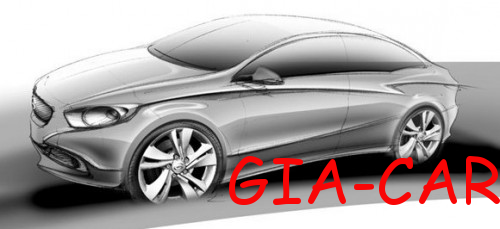
\includegraphics[width=0.7\linewidth]{./images/GIAcar}

\centering\Huge{Pflichtenheft} \\

\normalsize
\section*{Aufgabenbereiche}
	\begin{itemize}
	\item \textbf{Aktivitätsdiagramm, UseCase, Sequenzdiagramm:} Carlo, Sebastian, Martin
	\item \textbf{Server:} Max
	\item \textbf{OnlinePortale zum Projektmanagment Trello:} Bjarne, Timo, Quang
	\item \textbf{Versionsmanagement github:} Benedikt, Max, Noah
	\item \textbf{Scrum:} Daniel, Simon
	\item \textbf{Formalien, Dokumentation:} Noah, Suthe
	\end{itemize}
\section*{Programmiersprachen}
\begin{itemize}
\item html
\item css
\item javascript
\item php
\item bootstrap als html/css-framework
\end{itemize}
\section*{Software}
\begin{itemize}
\item ServerOS: Windows Server 2016
\item Webserver: apache2
\item php: Version 7
\item Datenbankserver: mysql
\item Dokumentation: latex
\item Bildberarbeitung: inkscape 
\item Analyse: piwik???
\end{itemize}



\end{document}
